\tikzstyle{input_neuron}=[circle,draw=black!50,fill=black!10,thick,minimum size=6mm]
\tikzstyle{hidden_neuron}=[circle,draw=blue!50,fill=blue!10,thick,minimum size=6mm]
\tikzstyle{output_neuron}=[circle,draw=green!50,fill=green!20,thick,minimum size=6mm]
\tikzstyle{hidden_neuron1}=[circle,draw=red!50,fill=red!10,thick,minimum size=6mm]
\tikzstyle{input}=[circle,draw=black!50,fill=black!20,thick,minimum size=6mm]

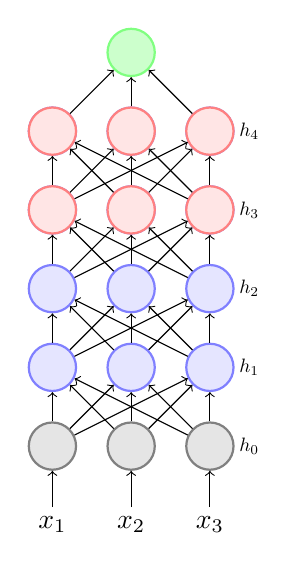
\begin{tikzpicture}
	
	\node [input_neuron] (in1) at (6,-2) {};
	\node [input_neuron] (in2) at (7,-2) {};
	\node [input_neuron] (in3) at (8,-2) {};
	\node [hidden_neuron] (h01) at (6,-1) {};
	\node [hidden_neuron] (h02) at (7,-1) {};
	\node [hidden_neuron] (h03) at (8,-1) {};
	\node [hidden_neuron] (h11) at (6,0) {};
	\node [hidden_neuron] (h12) at (7,0) {};
	\node [hidden_neuron] (h13) at (8,0) {};
	\node [hidden_neuron] (h21) at (6,1) {};
	\node [hidden_neuron] (h22) at (7,1) {};
	\node [hidden_neuron] (h23) at (8,1) {};
	\node [hidden_neuron] (h31) at (6,2) {};
	\node [hidden_neuron] (h32) at (7,2) {};
	\node [hidden_neuron] (h33) at (8,2) {};
	\node (input1) at (6,-3)  {$x_{1}$};
	\node (input2) at (7,-3)  {$x_{2}$};
	\node (input3) at (8,-3)  {$x_{3}$};
	\node [output_neuron] (o1) at (7,3) {};
	\draw [->] (input1) -- (in1);
	\draw [->] (input2) -- (in2);
	\draw [->] (input3) -- (in3);
	
	\draw [->] (in1) -- (h01);
	\draw [->] (in1) -- (h02);
	\draw [->] (in1) -- (h03);
	\draw [->] (in2) -- (h01);
	\draw [->] (in2) -- (h02);
	\draw [->] (in2) -- (h03);
	\draw [->] (in3) -- (h01);
	\draw [->] (in3) -- (h02);
	\draw [->] (in3) -- (h03);
	
	\draw [->] (h01) -- (h11);
	\draw [->] (h01) -- (h12);
	\draw [->] (h01) -- (h13);
	\draw [->] (h02) -- (h11);
	\draw [->] (h02) -- (h12);
	\draw [->] (h02) -- (h13);
	\draw [->] (h03) -- (h11);
	\draw [->] (h03) -- (h12);
	\draw [->] (h03) -- (h13);
	
	\draw [->] (h11) -- (h21);
	\draw [->] (h11) -- (h22);
	\draw [->] (h11) -- (h23);
	\draw [->] (h12) -- (h21);
	\draw [->] (h12) -- (h22);
	\draw [->] (h12) -- (h23);
	\draw [->] (h13) -- (h21);
	\draw [->] (h13) -- (h22);
	\draw [->] (h13) -- (h23);
	
	\draw [->] (h21) -- (h31);
	\draw [->] (h21) -- (h32);
	\draw [->] (h21) -- (h33);
	\draw [->] (h22) -- (h31);
	\draw [->] (h22) -- (h32);
	\draw [->] (h22) -- (h33);
	\draw [->] (h23) -- (h31);
	\draw [->] (h23) -- (h32);
	\draw [->] (h23) -- (h33);
	\draw [->] (h31) -- (o1);
	\draw [->] (h32) -- (o1);
	\draw [->] (h33) -- (o1);
	
	
	\node (formula)[scale=.7] at (8.5,-2) {$h_{0}$};
	
	\node (formula)[scale=.7] at (8.5,-1) {$h_{1}$};
	\node (formula)[scale=.7] at (8.5, 0) {$h_{2}$};
	\node (formula)[scale=.7] at (8.5,1) {$h_{3}$};
	\node (formula)[scale=.7] at (8.5,2) {$h_{4}$};
	
	\only<3->{
		\node [hidden_neuron1] (h21) at (6,1) {};
		\node [hidden_neuron1] (h22) at (7,1) {};
		\node [hidden_neuron1] (h23) at (8,1) {};
		\node [hidden_neuron1] (h31) at (6,2) {};
		\node [hidden_neuron1] (h32) at (7,2) {};
		\node [hidden_neuron1] (h33) at (8,2) {};
	}
	
\end{tikzpicture}